\documentclass[11pt]{beamer}
\usetheme{Madrid}
\usepackage{amsmath,amssymb,amsfonts,graphicx}
\usepackage{multicol,multirow,booktabs}
\usepackage{tikz}
\usepackage{pgfplots}
\pgfplotsset{compat=1.17}
\usepackage{siunitx}
\sisetup{output-decimal-marker={.},separate-uncertainty=true}

% To fit long frames
\setbeamerfont{normal text}{size=\small}

\title{H2 Physics \\ Potential Energy and Energy Conservation}
\author{R.F.H.}
\date{\today}

\begin{document}

\begin{frame}
\titlepage
\end{frame}

% Section 1: Getting Prepared
\section{Getting Prepared}

\begin{frame}[shrink=15]{Brain Dump}
\centering
\Large
\textit{What do you know about Potential Energy and Energy Conservation?}
\vfill
\end{frame}

\begin{frame}[shrink=15]{Brain Dump (CONT'D)}
\centering
\Large
\textit{What do you know about Potential Energy and Energy Conservation?}
\vfill
\begin{itemize}
    \item Gravitational potential energy near Earth: $E_p = mgh$
    \item Gravitational potential energy in space: $U = -\dfrac{GMm}{r}$
    \item Elastic potential energy: $E_e = \dfrac12 kx^2$
    \item Electric potential energy: $U_E = \dfrac{1}{4\pi\epsilon_0}\dfrac{Qq}{r}$
    \item Energy stored in a capacitor: $U = \dfrac12 QV = \dfrac12 CV^2$
    \item Work-energy theorem: $W_{\text{net}} = \Delta E_k$
    \item Conservation of mechanical energy: $E_k + E_p = \text{constant}$ (if no non-conservative forces)
    \item Power: $P = \dfrac{dE}{dt} = Fv$ (for constant force)
    \item Efficiency: $\eta = \dfrac{\text{useful energy output}}{\text{total energy input}}$
\end{itemize}
\end{frame}

\begin{frame}{Math Checklist}
Before tackling Energy, ensure you are comfortable with:
\begin{columns}[T]
\column{0.5\textwidth}
\begin{itemize}
    \item Solving quadratic equations
    \item Algebraic manipulation of formulas
    \item Integration (area under force-displacement graph)
    \item Differentiation (rate of change of energy)
\end{itemize}
\column{0.5\textwidth}
\begin{itemize}
    \item Trigonometric functions
    \item Logarithms and exponentials (for decay problems)
    \item Vector dot product (work = $\vec{F}\cdot\vec{s}$)
    \item Units and conversions (J, eV, kWh)
\end{itemize}
\end{columns}
\end{frame}

% Section 2: Concept Mastery
\section{Concept Mastery}

\begin{frame}{Building Intuition – Real-world Applications}
\begin{itemize}
    \item \alert{Roller coasters}: conversion between gravitational potential energy and kinetic energy.
    \item \alert{Pendulum}: energy oscillates between kinetic and potential.
    \item \alert{Bow and arrow}: elastic potential energy stored in limbs converted to kinetic energy of arrow.
    \item \alert{Hydroelectric dam}: gravitational potential energy of water converted to electrical energy.
    \item \alert{Satellite orbits}: total energy $E = -\frac{GMm}{2r}$ (negative indicates bound system).
    \item \alert{Capacitors}: energy stored in electric field.
    \item \alert{Nuclear reactions}: mass-energy equivalence $E = mc^2$.
\end{itemize}
\end{frame}

\begin{frame}{Formalization – Work and Energy}
\begin{block}{Work Done by a Constant Force}
$W = Fs\cos\theta$, where $\theta$ is angle between force and displacement.
\end{block}
\begin{block}{Kinetic Energy}
$E_k = \frac12 mv^2$
\end{block}
\begin{block}{Work-Energy Theorem}
$W_{\text{net}} = \Delta E_k$ (net work done on an object equals its change in kinetic energy)
\end{block}
\begin{block}{Conservation of Mechanical Energy}
If only conservative forces (gravity, spring force, electric force) do work,
\[ E_k + E_p = \text{constant} \]
\end{block}
\end{frame}

\begin{frame}{Formalization – Potential Energy Types}
\begin{itemize}
    \item \textbf{Gravitational potential energy (near Earth)}: $E_p = mgh$ (reference level at $h=0$)
    \item \textbf{Gravitational potential energy (general)}: $U = -\dfrac{GMm}{r}$ (zero at infinity)
    \item \textbf{Elastic potential energy}: $E_e = \dfrac12 kx^2$ (zero at natural length)
    \item \textbf{Electric potential energy (point charges)}: $U_E = \dfrac{1}{4\pi\epsilon_0}\dfrac{Qq}{r}$ (zero at infinity)
    \item \textbf{Energy stored in a capacitor}: $U = \dfrac12 QV = \dfrac12 CV^2 = \dfrac12 \dfrac{Q^2}{C}$
\end{itemize}
\end{frame}

\begin{frame}{Formalization – Power and Efficiency}
\begin{block}{Power}
Rate of energy transfer: $P = \dfrac{dE}{dt}$.
For constant force and velocity: $P = Fv\cos\theta$.
\end{block}
\begin{block}{Efficiency}
\[ \eta = \frac{\text{useful energy output}}{\text{total energy input}} \times 100\% \]
Energy losses often due to friction, heat, sound, etc.
\end{block}
\end{frame}

\begin{frame}{Micro-Testing – Quick Checks}
\begin{enumerate}
    \item A ball of mass $2\ \mathrm{kg}$ is dropped from height $10\ \mathrm{m}$. What is its speed just before hitting ground? \pause \alert{$v = \sqrt{2gh} = \sqrt{2\times9.81\times10} \approx 14.0\ \mathrm{m/s}$}.
    \item A spring of constant $k = 500\ \mathrm{N/m}$ is compressed by $0.1\ \mathrm{m}$. How much energy is stored? \pause \alert{$E = \frac12 kx^2 = 0.5\times500\times0.01 = 2.5\ \mathrm{J}$}.
    \item A force of $10\ \mathrm{N}$ acts at $60^\circ$ to displacement of $5\ \mathrm{m}$. Work done? \pause \alert{$W = Fs\cos60^\circ = 10\times5\times0.5 = 25\ \mathrm{J}$}.
    \item A satellite orbits Earth. Its total energy is negative. What does that indicate? \pause \alert{It is bound to Earth; would need energy input to escape}.
    \item A motor lifts a $50\ \mathrm{kg}$ mass at constant speed $2\ \mathrm{m/s}$. What power is needed (ignoring losses)? \pause \alert{$P = Fv = mgv = 50\times9.81\times2 = 981\ \mathrm{W}$}.
\end{enumerate}
\end{frame}

% Section 3: Past Problems
\section{Past Problems}

% ------------------------------------------------
% Paper 1 Questions
% ------------------------------------------------
\subsection{Paper 1}

% NJC 2025 P1 Q5
\begin{frame}[shrink=15]{NJC 2025 H2 Physics Prelim Paper 1 Q5}
Two frictionless trolleys move along the same straight line towards one another. Masses and velocities before collision are shown. The trolleys collide and stick together. What is the final kinetic energy of the trolleys after the collision?
\begin{center}
( Diagram: 5.0 kg at 4.0 m/s right, 2.0 kg at 3.0 m/s left )
\end{center}
\begin{enumerate}[A]
    \item $0.71\ \mathrm{J}$
    \item $14\ \mathrm{J}$
    \item $31\ \mathrm{J}$
    \item $35\ \mathrm{J}$
\end{enumerate}
\end{frame}

\begin{frame}{NJC 2025 P1 Q5 – Solution}
Conservation of momentum (right positive):
\[ (5.0)(4.0) + (2.0)(-3.0) = (5.0+2.0)v \]
\[ 20.0 - 6.0 = 7.0v \Rightarrow v = 2.0\ \mathrm{m/s} \]
Final kinetic energy:
\[ E_k = \frac12 (7.0)(2.0)^2 = 0.5\times7.0\times4 = 14\ \mathrm{J} \]
Answer: \textbf{B}.
\end{frame}

% NJC 2025 P1 Q8
\begin{frame}[shrink=15]{NJC 2025 H2 Physics Prelim Paper 1 Q8}
A turbine at a hydroelectric power station is situated at a vertical distance $30\ \mathrm{m}$ below the surface of a large lake. Water passes through the turbine at $5.7\ \mathrm{m^3/s}$. Overall efficiency $90\%$, density of water $1000\ \mathrm{kg/m^3}$. What is the useful power output?
\begin{enumerate}[A]
    \item $0.15\ \mathrm{MW}$
    \item $1.5\ \mathrm{MW}$
    \item $1.7\ \mathrm{MW}$
    \item $90\ \mathrm{MW}$
\end{enumerate}
\end{frame}

\begin{frame}{NJC 2025 P1 Q8 – Solution}
Mass flow rate: $\dot{m} = \rho \times \text{volume flow rate} = 1000\times5.7 = 5700\ \mathrm{kg/s}$.
Power available from falling water: $P_{\text{in}} = \dot{m} g h = 5700\times9.81\times30$.
$P_{\text{in}} = 5700\times294.3 = 1\,677\,510\ \mathrm{W} \approx 1.68\ \mathrm{MW}$.
Useful power $= 0.90 \times 1.68 = 1.51\ \mathrm{MW} \approx 1.5\ \mathrm{MW}$.
Answer: \textbf{B}.
\end{frame}

% NJC 2025 P1 Q12
\begin{frame}[shrink=15]{NJC 2025 H2 Physics Prelim Paper 1 Q12}
A huge block of ice at $0^\circ\mathrm{C}$ with a hollow in its top surface. A mass of $160\ \mathrm{g}$ of water at $100^\circ\mathrm{C}$ is poured into the hollow. Specific heat capacity of water $4.20\ \mathrm{kJ\,kg^{-1}K^{-1}}$, latent heat of fusion of ice $336\ \mathrm{kJ\,kg^{-1}}$. After thermal equilibrium, what is the total mass of water in the hollow?
\begin{enumerate}[A]
    \item $100\ \mathrm{g}$
    \item $200\ \mathrm{g}$
    \item $260\ \mathrm{g}$
    \item $360\ \mathrm{g}$
\end{enumerate}
\end{frame}

\begin{frame}{NJC 2025 P1 Q12 – Solution}
Heat lost by hot water cooling to $0^\circ\mathrm{C}$: $Q = mc\Delta T = 0.160\times4200\times100 = 67200\ \mathrm{J}$.
This heat melts ice: mass melted $= \frac{Q}{L} = \frac{67200}{336000} = 0.200\ \mathrm{kg} = 200\ \mathrm{g}$.
Total water in hollow = original $160\ \mathrm{g}$ + melted $200\ \mathrm{g} = 360\ \mathrm{g}$.
Answer: \textbf{D}.
\end{frame}

% NJC 2025 P1 Q20
\begin{frame}[shrink=15]{NJC 2025 H2 Physics Prelim Paper 1 Q20}
An alpha particle with kinetic energy $9.0\times10^{-13}\ \mathrm{J}$ approaches a stationary gold nucleus ($79$ protons). Find the closest possible distance of approach.
\begin{enumerate}[A]
    \item $2.5\times10^{-16}\ \mathrm{m}$
    \item $2.0\times10^{-14}\ \mathrm{m}$
    \item $4.0\times10^{-14}\ \mathrm{m}$
    \item $2.0\times10^{-7}\ \mathrm{m}$
\end{enumerate}
\end{frame}

\begin{frame}{NJC 2025 P1 Q20 – Solution}
At closest approach, kinetic energy is converted to electric potential energy:
\[ \frac12 m v^2 = \frac{1}{4\pi\epsilon_0}\frac{Q_{\alpha} Q_{\text{Au}}}{r} \]
$Q_{\alpha} = 2e$, $Q_{\text{Au}} = 79e$.
\[ 9.0\times10^{-13} = \frac{(8.99\times10^9)(2\times1.60\times10^{-19})(79\times1.60\times10^{-19})}{r} \]
Numerator: $8.99\times10^9 \times 3.2\times10^{-19} \times 1.264\times10^{-17} = 8.99\times10^9 \times 4.0448\times10^{-36} = 3.637\times10^{-26}$.
Thus $r = \frac{3.637\times10^{-26}}{9.0\times10^{-13}} = 4.04\times10^{-14}\ \mathrm{m} \approx 4.0\times10^{-14}\ \mathrm{m}$.
Answer: \textbf{C}.
\end{frame}

% NYJC 2025 P1 Q8
\begin{frame}[shrink=15]{NYJC 2025 H2 Physics Prelim Paper 1 Q8}
A wire is stretched elastically by a force of $200\ \mathrm{N}$, causing an extension of $2.00\ \mathrm{mm}$. The force is gradually increased to $250\ \mathrm{N}$, wire remains elastic. What is the work done in stretching from $200\ \mathrm{N}$ to $250\ \mathrm{N}$?
\begin{enumerate}[A]
    \item $0.113\ \mathrm{J}$
    \item $0.225\ \mathrm{J}$
    \item $113\ \mathrm{J}$
    \item $225\ \mathrm{J}$
\end{enumerate}
\end{frame}

\begin{frame}{NYJC 2025 P1 Q8 – Solution}
Spring constant $k = \frac{F}{x} = \frac{200}{0.002} = 100000\ \mathrm{N/m}$.
Extension at $250\ \mathrm{N}$: $x_2 = \frac{250}{100000} = 0.0025\ \mathrm{m}$.
Work done = area under force-extension graph (trapezoid):
\[ W = \frac12 (200 + 250)(0.0025 - 0.002) = 0.5\times450\times0.0005 = 0.1125\ \mathrm{J} \approx 0.113\ \mathrm{J} \]
Answer: \textbf{A}.
\end{frame}

% RI 2025 P1 Q4
\begin{frame}[shrink=15]{RI 2025 H2 Physics Prelim Paper 1 Q4}
The force $F$ required to extend a spring of unstretched length $x_0$ to length $x$ is measured. When tension is $T_1$, length is $x_1$; when tension $T_2$, length $x_2$. What is the work done to stretch from $x_1$ to $x_2$?
\begin{enumerate}[A]
    \item $\frac12 T_2(x_2 - x_0)$
    \item $\frac12 (T_1 + T_2)(x_2 - x_1)$
    \item $\frac12 (T_1 + T_2)(x_2 + x_1 - 2x_0)$
    \item $\frac12 (T_1 + T_2)(x_2 - x_1 - 2x_0)$
\end{enumerate}
\end{frame}

\begin{frame}{RI 2025 P1 Q4 – Solution}
Work done = area under force-extension graph. Extension is $(x - x_0)$. At $x_1$, extension $e_1 = x_1 - x_0$; at $x_2$, extension $e_2 = x_2 - x_0$.
Work = area of trapezoid under force vs extension:
\[ W = \frac12 (T_1 + T_2)(e_2 - e_1) = \frac12 (T_1 + T_2)[(x_2 - x_0) - (x_1 - x_0)] = \frac12 (T_1 + T_2)(x_2 - x_1) \]
Answer: \textbf{B}.
\end{frame}

% HCI 2025 P1 Q7
\begin{frame}[shrink=15]{HCI 2025 H2 Physics Prelim Paper 1 Q7}
A driving force of $250\ \mathrm{N}$ is needed for a car of mass $900\ \mathrm{kg}$ to travel along a level road at constant speed $24\ \mathrm{m/s}$. What power is required to maintain this speed when moving up a slope that rises $1.0\ \mathrm{m}$ for every $12\ \mathrm{m}$ of travel?
\begin{enumerate}[A]
    \item $6.8\ \mathrm{kW}$
    \item $12\ \mathrm{kW}$
    \item $18\ \mathrm{kW}$
    \item $24\ \mathrm{kW}$
\end{enumerate}
\end{frame}

\begin{frame}{HCI 2025 P1 Q7 – Solution}
On slope, component of weight down slope $= mg\sin\theta$, with $\sin\theta = \frac{1}{12}$.
Total force required $= 250 + 900\times9.81\times\frac{1}{12} = 250 + 8829/12 = 250 + 735.75 = 985.75\ \mathrm{N}$.
Power $= Fv = 985.75\times24 = 23658\ \mathrm{W} \approx 23.7\ \mathrm{kW}$.
Closest answer: \textbf{D} (24 kW).
\end{frame}

% ------------------------------------------------
% Paper 2 Questions
% ------------------------------------------------
\subsection{Paper 2}

% NJC 2025 P2 Q1
\begin{frame}[shrink=15]{NJC 2025 H2 Physics Prelim Paper 2 Q1}
A pellet of mass $8.00\times10^{-3}\ \mathrm{kg}$ is projected at angle $\theta$ above horizontal with speed $u$. It reaches maximum height $10.0\ \mathrm{m}$ and speed $5.00\ \mathrm{m/s}$ at maximum height. Air resistance negligible.
\begin{itemize}
    \item[(a)(i)] Show $u = 14.9\ \mathrm{m/s}$ using energy conservation.
    \item[(a)(ii)] Calculate $\theta$.
\end{itemize}
\end{frame}

\begin{frame}{NJC 2025 P2 Q1 – Solution (i)}
At max height, vertical velocity zero, so speed $= u\cos\theta = 5.00$.
Energy conservation: loss in KE = gain in GPE.
\[ \frac12 m u^2 - \frac12 m (5.00)^2 = m g (10.0) \]
Cancel $m$: $\frac12 u^2 - \frac12 (25) = 98.1$
\[ 0.5 u^2 = 98.1 + 12.5 = 110.6 \Rightarrow u^2 = 221.2 \Rightarrow u \approx 14.87\ \mathrm{m/s} \approx 14.9\ \mathrm{m/s} \]
\end{frame}

\begin{frame}{NJC 2025 P2 Q1 – Solution (ii)}
From $u\cos\theta = 5.00$, $\cos\theta = \frac{5.00}{14.87} \approx 0.3362$, $\theta \approx 70.4^\circ$.
\end{frame}

% NYJC 2025 P2 Q2 (ballistic pendulum)
\begin{frame}[shrink=15]{NYJC 2025 H2 Physics Prelim Paper 2 Q2}
A bullet of mass $2.0\ \mathrm{g}$ is fired horizontally into a block of wood of mass $600\ \mathrm{g}$ suspended by strings. The bullet embeds, and the block rises $8.6\ \mathrm{cm}$. 
\begin{itemize}
    \item[(b)(i)] Show speed of block+bullet just after impact is $1.3\ \mathrm{m/s}$.
    \item[(b)(ii)] Find speed of bullet before impact.
\end{itemize}
\end{frame}

\begin{frame}{NYJC 2025 P2 Q2 – Solution (i)}
After impact, kinetic energy converts to gravitational potential energy:
\[ \frac12 (0.602) v^2 = (0.602) g (0.086) \]
Cancel $0.602$: $\frac12 v^2 = 9.81\times0.086 = 0.84366$
\[ v^2 = 1.68732 \Rightarrow v \approx 1.299\ \mathrm{m/s} \approx 1.3\ \mathrm{m/s} \]
\end{frame}

\begin{frame}{NYJC 2025 P2 Q2 – Solution (ii)}
Conservation of momentum during collision:
\[ 0.002\, u = 0.602 \times 1.299 \]
\[ u = \frac{0.602\times1.299}{0.002} = \frac{0.782}{0.002} = 391\ \mathrm{m/s} \]
\end{frame}

% HCI 2025 P2 Q8(a) (ski lift power)
\begin{frame}[shrink=15]{HCI 2025 H2 Physics Prelim Paper 2 Q8(a)}
A ski lift uses 48 two-person chairs, each mass $80\ \mathrm{kg}$, moving at $2.5\ \mathrm{m/s}$ up a height of $300\ \mathrm{m}$ over a distance $900\ \mathrm{m}$. Average skier mass $75\ \mathrm{kg}$. Calculate mechanical power required.
\end{frame}

\begin{frame}{HCI 2025 P2 Q8(a) – Solution}
Number of skiers per chair = 2, so total skiers $= 48\times2 = 96$.
Total mass of skiers $= 96\times75 = 7200\ \mathrm{kg}$. Total mass of chairs $= 48\times80 = 3840\ \mathrm{kg}$. Total mass $= 11040\ \mathrm{kg}$.
Time to travel $900\ \mathrm{m}$ at $2.5\ \mathrm{m/s}$: $t = 900/2.5 = 360\ \mathrm{s}$.
Power = rate of gain of gravitational potential energy:
\[ P = \frac{mgh}{t} = \frac{11040\times9.81\times300}{360} \]
$11040\times9.81 = 108302.4$, times $300 = 32490720$, divide by $360 = 90252\ \mathrm{W} \approx 90.3\ \mathrm{kW}$.
\end{frame}

% RI 2025 P2 Q3 (yoke SHM energy)
\begin{frame}[shrink=15]{RI 2025 H2 Physics Prelim Paper 2 Q3}
A yoke of mass $0.30\ \mathrm{kg}$ moves with SHM, amplitude $0.080\ \mathrm{m}$, period $0.40\ \mathrm{s}$. Determine maximum speed and maximum acceleration. Then sketch net force vs time. (Energy not explicitly asked, but we can extract energy.)
\end{frame}

\begin{frame}{RI 2025 P2 Q3 – Energy Extraction}
Maximum speed $v_0 = \omega r = \frac{2\pi}{0.40}\times0.080 = 15.708\times0.08 = 1.2566\ \mathrm{m/s}$.
Maximum kinetic energy $= \frac12 m v_0^2 = 0.5\times0.30\times(1.2566)^2 = 0.15\times1.579 = 0.237\ \mathrm{J}$.
This equals total energy of oscillation.
\end{frame}

% ------------------------------------------------
% Paper 3 Questions
% ------------------------------------------------
\subsection{Paper 3}

% NJC 2025 P3 Q1 (gravitational potential energy)
\begin{frame}[shrink=15]{NJC 2025 H2 Physics Prelim Paper 3 Q1}
The Earth radius $R = 6.4\times10^6\ \mathrm{m}$, mass $M = 6.0\times10^{24}\ \mathrm{kg}$. A meteorite falls from rest at a great distance. Find its speed when at distance $3R$ from Earth's centre. (Use graph of $\phi$ vs $x$.)
\end{frame}

\begin{frame}{NJC 2025 P3 Q1 – Solution}
Gravitational potential at infinity $=0$, at $3R$: from graph, $\phi \approx -2.1\times10^7\ \mathrm{J/kg}$.
Conservation of energy: $0 = \frac12 v^2 + \phi \Rightarrow v = \sqrt{-2\phi} = \sqrt{4.2\times10^7} \approx 6481\ \mathrm{m/s}$.
\end{frame}

% NYJC 2025 P3 Q3 (escape velocity, energy)
\begin{frame}[shrink=15]{NYJC 2025 H2 Physics Prelim Paper 3 Q3}
Planet Z has density $\rho$ and radius $r$. Show escape velocity $v = \sqrt{\frac83 G\pi\rho r^2}$. Given $\rho = 5500\ \mathrm{kg/m^3}$, $r = 413\ \mathrm{km}$, calculate $v$. Then find temperature of atmosphere if $v = c_{\text{rms}}$.
\end{frame}

\begin{frame}{NYJC 2025 P3 Q3 – Solution (a)}
Escape velocity: $\frac12 m v^2 = \frac{GMm}{r}$, with $M = \frac43 \pi r^3 \rho$.
Thus $v^2 = \frac{2G}{r} \cdot \frac43 \pi r^3 \rho = \frac83 G\pi \rho r^2$, so $v = \sqrt{\frac83 G\pi \rho r^2}$.
\end{frame}

\begin{frame}{NYJC 2025 P3 Q3 – Solution (b)}
$v = \sqrt{\frac83 (6.67\times10^{-11})\pi (5500)(413\times10^3)^2}$.
First compute $r^2 = (4.13\times10^5)^2 = 1.706\times10^{11}$.
$\rho r^2 = 5500\times1.706\times10^{11} = 9.383\times10^{14}$.
$G\pi \rho r^2 = 6.67\times10^{-11}\times\pi\times9.383\times10^{14} = 6.67\times10^{-11}\times2.947\times10^{15} = 1.966\times10^5$.
$\frac83$ of that $= 2.6667\times1.966\times10^5 = 5.243\times10^5$.
$v = \sqrt{5.243\times10^5} \approx 724\ \mathrm{m/s}$.
\end{frame}

\begin{frame}{NYJC 2025 P3 Q3 – Solution (c)}
$c_{\text{rms}} = v = \sqrt{\frac{3RT}{M}}$ where $M$ is molar mass ($40\ \mathrm{g/mol} = 0.040\ \mathrm{kg/mol}$).
$T = \frac{M v^2}{3R} = \frac{0.040\times(724)^2}{3\times8.31} = \frac{0.040\times524176}{24.93} = \frac{20967}{24.93} \approx 841\ \mathrm{K}$.
\end{frame}

% HCI 2025 P3 Q1 (projectile energy)
\begin{frame}[shrink=15]{HCI 2025 H2 Physics Prelim Paper 3 Q1}
A ball is thrown at $25\ \mathrm{m/s}$, $30^\circ$. Find max height, and at that height express KE and PE in terms of initial KE $K$.
\end{frame}

\begin{frame}{HCI 2025 P3 Q1 – Solution}
$u_y = 25\sin30^\circ = 12.5\ \mathrm{m/s}$. Max height $h = \frac{u_y^2}{2g} = \frac{156.25}{19.62} = 7.96\ \mathrm{m}$.
At top, speed $= u_x = 25\cos30^\circ = 21.65\ \mathrm{m/s}$, so KE $= \frac12 m (21.65)^2 = \frac12 m u^2 \left(\frac{21.65}{25}\right)^2 = K \times 0.75$.
PE $= mgh = mg(7.96) = \frac12 m u^2 \times \frac{2gh}{u^2} = K \times \frac{2\times9.81\times7.96}{625} = K \times \frac{156.2}{625} = K \times 0.25$.
So KE = $0.75K$, PE = $0.25K$.
\end{frame}

% RI 2025 P3 Q3 (projectile energy)
\begin{frame}[shrink=15]{RI 2025 H2 Physics Prelim Paper 3 Q3}
An archer fires an arrow at $52\ \mathrm{m/s}$, $15^\circ$ from height $1.5\ \mathrm{m}$. It hits a tree at height $8.0\ \mathrm{m}$. Find KE just before impact and distance to tree.
\end{frame}

\begin{frame}{RI 2025 P3 Q3 – Solution (KE)}
Energy conservation: $\frac12 m v_i^2 = \frac12 m v_f^2 + mg(8.0-1.5)$.
$\frac12 v_f^2 = \frac12 (52)^2 - 9.81\times6.5 = 1352 - 63.765 = 1288.235$.
$v_f^2 = 2576.47$, $v_f \approx 50.76\ \mathrm{m/s}$.
KE $= \frac12 m (50.76)^2$. With $m=0.032\ \mathrm{kg}$, KE $= 0.5\times0.032\times2576.47 = 0.016\times2576.47 = 41.22\ \mathrm{J}$.
\end{frame}

\begin{frame}{RI 2025 P3 Q3 – Solution (distance)}
$u_x = 52\cos15^\circ \approx 50.24\ \mathrm{m/s}$, $u_y = 52\sin15^\circ \approx 13.46\ \mathrm{m/s}$.
Vertical motion: $s_y = u_y t - \frac12 g t^2$, $s_y = 6.5\ \mathrm{m}$.
$6.5 = 13.46 t - 4.905 t^2 \Rightarrow 4.905 t^2 - 13.46 t + 6.5 = 0$.
Solve: $t = \frac{13.46 \pm \sqrt{181.17 - 127.53}}{9.81} = \frac{13.46 \pm 7.324}{9.81}$.
$t = 0.626\ \mathrm{s}$ (on way up) or $2.12\ \mathrm{s}$ (down). Use $t=0.626$.
$x = u_x t = 50.24\times0.626 \approx 31.4\ \mathrm{m}$.
\end{frame}

% Section 4: Question Bank
\section{Question Bank}

\subsection{Gravitational Potential Energy (H2 Level)}

\begin{frame}[shrink=15]{Variation 1 – Falling Object \hfill Difficulty: 2/10}
A stone of mass $0.5\ \mathrm{kg}$ is dropped from a height of $20\ \mathrm{m}$. Find its speed just before hitting the ground.
\end{frame}

\begin{frame}{Variation 1 – Solution}
$v = \sqrt{2gh} = \sqrt{2\times9.81\times20} = \sqrt{392.4} \approx 19.8\ \mathrm{m/s}$.
\end{frame}

\begin{frame}[shrink=15]{Variation 2 – Roller Coaster \hfill Difficulty: 3/10}
A roller coaster car starts from rest at height $h$ above the bottom of a frictionless loop of radius $R$. What minimum $h$ is needed for the car to just make it around the loop?
\end{frame}

\begin{frame}{Variation 2 – Solution}
At top of loop, need $v \ge \sqrt{gR}$. Energy conservation: $mgh = mg(2R) + \frac12 m gR = \frac52 mgR$, so $h = \frac52 R$.
\end{frame}

\begin{frame}[shrink=15]{Variation 3 – Satellite Energy \hfill Difficulty: 4/10}
A satellite of mass $500\ \mathrm{kg}$ orbits Earth at a height of $300\ \mathrm{km}$. Earth mass $M = 6.0\times10^{24}\ \mathrm{kg}$, radius $R = 6.37\times10^6\ \mathrm{m}$, $G = 6.67\times10^{-11}$. Find its total mechanical energy.
\end{frame}

\begin{frame}{Variation 3 – Solution}
Orbital radius $r = R + h = 6.37\times10^6 + 3.0\times10^5 = 6.67\times10^6\ \mathrm{m}$.
Total energy $E = -\frac{GMm}{2r} = -\frac{6.67\times10^{-11}\times6.0\times10^{24}\times500}{2\times6.67\times10^6}$.
$GMm = 6.67\times10^{-11}\times6.0\times10^{24}\times500 = 2.001\times10^{17}$.
Divide by $2r = 1.334\times10^7$: $E = -1.5\times10^{10}\ \mathrm{J}$.
\end{frame}

\subsection{Elastic Potential Energy (H2 Level)}

\begin{frame}[shrink=15]{Variation 4 – Spring Compression \hfill Difficulty: 3/10}
A spring with $k = 800\ \mathrm{N/m}$ is compressed by $0.15\ \mathrm{m}$. How much energy is stored? If a $0.2\ \mathrm{kg}$ mass is placed against it and released, what speed does the mass have when the spring returns to natural length?
\end{frame}

\begin{frame}{Variation 4 – Solution}
$E_e = \frac12 k x^2 = 0.5\times800\times0.0225 = 9\ \mathrm{J}$.
$v = \sqrt{\frac{2E_e}{m}} = \sqrt{\frac{18}{0.2}} = \sqrt{90} \approx 9.49\ \mathrm{m/s}$.
\end{frame}

\begin{frame}[shrink=15]{Variation 5 – Two Springs in Parallel \hfill Difficulty: 4/10}
Two identical springs of constant $k = 300\ \mathrm{N/m}$ are connected in parallel. A mass of $2\ \mathrm{kg}$ is attached and displaced $0.1\ \mathrm{m}$ from equilibrium. Find the total energy stored.
\end{frame}

\begin{frame}{Variation 5 – Solution}
Effective $k_{\text{eff}} = 2k = 600\ \mathrm{N/m}$. Energy $= \frac12 k_{\text{eff}} x^2 = 0.5\times600\times0.01 = 3\ \mathrm{J}$.
\end{frame}

\subsection{Electric Potential Energy (H2 Level)}

\begin{frame}[shrink=15]{Variation 6 – Point Charges \hfill Difficulty: 5/10}
Two point charges $Q_1 = +3\ \mu\mathrm{C}$ and $Q_2 = -2\ \mu\mathrm{C}$ are initially $0.5\ \mathrm{m}$ apart. How much work is required to separate them to $1.0\ \mathrm{m}$?
\end{frame}

\begin{frame}{Variation 6 – Solution}
Initial potential energy: $U_i = \frac{1}{4\pi\epsilon_0} \frac{Q_1 Q_2}{r_i} = 8.99\times10^9 \times \frac{(3\times10^{-6})(-2\times10^{-6})}{0.5} = 8.99\times10^9 \times \frac{-6\times10^{-12}}{0.5} = 8.99\times10^9 \times (-1.2\times10^{-11}) = -0.1079\ \mathrm{J}$.
Final: $U_f = 8.99\times10^9 \times \frac{-6\times10^{-12}}{1.0} = -0.05394\ \mathrm{J}$.
Work done by external force = $\Delta U = U_f - U_i = -0.05394 - (-0.1079) = 0.05396\ \mathrm{J}$.
\end{frame}

\subsection{Energy in Capacitors (H2 Level)}

\begin{frame}[shrink=15]{Variation 7 – Capacitor Energy \hfill Difficulty: 3/10}
A $100\ \mu\mathrm{F}$ capacitor is charged to $50\ \mathrm{V}$. How much energy is stored? If discharged through a resistor, how much heat is dissipated?
\end{frame}

\begin{frame}{Variation 7 – Solution}
$U = \frac12 CV^2 = 0.5\times100\times10^{-6}\times2500 = 0.125\ \mathrm{J}$. All this energy becomes heat.
\end{frame}

\subsection{Work and Power (H2 Level)}

\begin{frame}[shrink=15]{Variation 8 – Constant Force \hfill Difficulty: 2/10}
A force of $30\ \mathrm{N}$ pushes a box $5\ \mathrm{m}$ across a floor. How much work is done? If the force is applied at $40^\circ$ to the horizontal, what is the work?
\end{frame}

\begin{frame}{Variation 8 – Solution}
$W = Fs = 30\times5 = 150\ \mathrm{J}$. With angle: $W = Fs\cos40^\circ = 150\times0.7660 = 114.9\ \mathrm{J}$.
\end{frame}

\begin{frame}[shrink=15]{Variation 9 – Power of Motor \hfill Difficulty: 3/10}
A motor lifts a $200\ \mathrm{kg}$ crate at constant speed $1.5\ \mathrm{m/s}$. What is the power output of the motor?
\end{frame}

\begin{frame}{Variation 9 – Solution}
$P = Fv = mgv = 200\times9.81\times1.5 = 2943\ \mathrm{W} \approx 2.94\ \mathrm{kW}$.
\end{frame}

\begin{frame}[shrink=15]{Variation 10 – Efficiency \hfill Difficulty: 4/10}
An electric motor has an efficiency of $85\%$. It lifts a $50\ \mathrm{kg}$ mass through $10\ \mathrm{m}$ in $5\ \mathrm{s}$. What electrical power is drawn?
\end{frame}

\begin{frame}{Variation 10 – Solution}
Useful power $= \frac{mgh}{t} = \frac{50\times9.81\times10}{5} = \frac{4905}{5} = 981\ \mathrm{W}$.
Electrical power $= \frac{981}{0.85} \approx 1154\ \mathrm{W}$.
\end{frame}

\subsection{Challenge Problems (H3 / Competition)}

\begin{frame}[shrink=15]{Challenge 1 – Loop with Friction \hfill Difficulty: 8/10}
A block starts from rest at height $h$ above the bottom of a loop of radius $R$. The track has coefficient of kinetic friction $\mu$ on the horizontal approach only. Find $h$ such that the block just makes it around the loop.
\end{frame}

\begin{frame}{Challenge 1 – Solution}
Speed needed at top: $v_{\text{top}} = \sqrt{gR}$. Energy from start to top: $mgh = mg(2R) + \frac12 m gR + \mu mg d$, where $d$ is horizontal distance before loop. So $h = \frac52 R + \mu d$.
\end{frame}

\begin{frame}[shrink=15]{Challenge 2 – Mass on String with Variable Length \hfill Difficulty: 9/10}
A mass attached to a string is rotated in a horizontal circle. The string is slowly pulled down through a hole, reducing radius. If initial radius $r_0$ and angular velocity $\omega_0$, find final angular velocity when radius is $r_f$. (Energy not conserved because tension does work.)
\end{frame}

\begin{frame}{Challenge 2 – Solution}
Angular momentum $L = m r^2 \omega$ is conserved (torque zero about centre). So $r^2 \omega = \text{constant}$, thus $\omega_f = \omega_0 (r_0/r_f)^2$. Energy is not conserved because work is done pulling the string.
\end{frame}

\begin{frame}[shrink=15]{Challenge 3 – Gravitational Slingshot \hfill Difficulty: 9/10}
A spacecraft approaches a planet of mass $M$ with speed $v_0$ (relative to planet) and impact parameter $b$. Derive the condition for it to gain energy from the encounter.
\end{frame}

\begin{frame}{Challenge 3 – Solution}
In planet's frame, spacecraft's speed is unchanged (elastic collision with planet), but direction changes. In Sun's frame, if planet is moving, the spacecraft can gain or lose energy. Maximum gain when spacecraft approaches from behind and exits ahead. Analysis uses conservation of energy and angular momentum in planet's frame, then transforming back.
\end{frame}

\begin{frame}[shrink=15]{Challenge 4 – Electric Potential Energy of System \hfill Difficulty: 8/10}
Four equal positive charges $q$ are placed at corners of a square of side $a$. Find the total electric potential energy of the system.
\end{frame}

\begin{frame}{Challenge 4 – Solution}
There are $6$ pairs. For adjacent corners: distance $a$, energy per pair $= \frac{1}{4\pi\epsilon_0}\frac{q^2}{a}$, 4 such pairs. For diagonal pairs: distance $a\sqrt{2}$, energy per pair $= \frac{1}{4\pi\epsilon_0}\frac{q^2}{a\sqrt{2}}$, 2 such pairs. Total $U = \frac{1}{4\pi\epsilon_0}\frac{q^2}{a}\left(4 + \frac{2}{\sqrt{2}}\right) = \frac{1}{4\pi\epsilon_0}\frac{q^2}{a}\left(4 + \sqrt{2}\right)$.
\end{frame}

\begin{frame}[shrink=15]{Challenge 5 – Energy in Charging a Capacitor \hfill Difficulty: 7/10}
A capacitor $C$ is charged through a resistor $R$ from a battery of emf $V$. Show that the energy supplied by the battery is twice the energy stored in the capacitor, and explain where the other half goes.
\end{frame}

\begin{frame}{Challenge 5 – Solution}
Energy from battery $= \int V I dt = V \int I dt = V Q = V (CV) = CV^2$.
Energy stored in capacitor $= \frac12 CV^2$.
The other half is dissipated as heat in the resistor. This can be shown by integrating $I^2 R$ over time.
\end{frame}

% Section 5: Synthesis & Consolidation
\section{Synthesis \& Consolidation}

\begin{frame}{End‑of‑Session Concept Recap}
\begin{itemize}
    \item Energy is a scalar quantity, conserved in isolated systems.
    \item Work done by conservative forces is path-independent and stored as potential energy.
    \item Gravitational potential energy: $mgh$ (near Earth) or $-\frac{GMm}{r}$ (general).
    \item Elastic potential energy: $\frac12 kx^2$.
    \item Electric potential energy: $\frac{1}{4\pi\epsilon_0}\frac{Qq}{r}$.
    \item Energy in capacitor: $\frac12 CV^2$.
    \item Power: rate of energy transfer, $P = Fv$ for constant force.
    \item Efficiency accounts for energy losses.
\end{itemize}
\end{frame}

\begin{frame}{Mind Map}
\centering
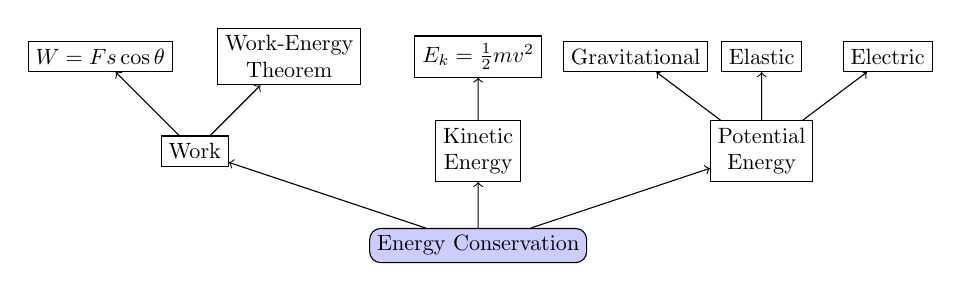
\begin{tikzpicture}[scale=0.8, transform shape]

% Root Node
\node[draw,rounded corners,fill=blue!20] (root) at (0,0) {Energy Conservation};

% Level 1: Categories
\node[draw] (work) at (-4.5,1.5) {Work};
\node[draw, align=center] (ke) at (0,1.5) {Kinetic \\ Energy};
\node[draw, align=center] (pe) at (4.5,1.5) {Potential \\ Energy};

% Level 2: Equations & Types
% Children of Work
\node[draw] (w_eq) at (-6,3) {$W = Fs\cos\theta$};
\node[draw, align=center] (we_thm) at (-3,3) {Work-Energy \\ Theorem};

% Child of Kinetic Energy
\node[draw] (ke_eq) at (0,3) {$E_k = \frac12 mv^2$};

% Children of Potential Energy
\node[draw] (grav) at (2.5,3) {Gravitational};
\node[draw] (elast) at (4.5,3) {Elastic};
\node[draw] (elec) at (6.5,3) {Electric};

% Arrows (Root to Level 1)
\draw[->] (root) -- (work);
\draw[->] (root) -- (ke);
\draw[->] (root) -- (pe);

% Arrows (Level 1 to Level 2)
\draw[->] (work) -- (w_eq);
\draw[->] (work) -- (we_thm);

\draw[->] (ke) -- (ke_eq);

\draw[->] (pe) -- (grav);
\draw[->] (pe) -- (elast);
\draw[->] (pe) -- (elec);

\end{tikzpicture}
\vfill
Link to dynamics: forces do work, changing energy. Link to thermal: energy dissipation. Link to circuits: energy in capacitors and batteries.
\end{frame}

\end{document}